% M3 Comparison Part (Emmanuel Omole, 101004432).
% \input{} into the IEEE conference report. Needs graphicx.
% Subsections map to the M3 headings; move them into the group sections.

\subsection{Methods executed: Comparison Part}

\textbf{Data.} AEEEM: EQ (324 classes, 39.8\% defective), JDT (997, 20.7\%),
LC (691, 9.3\%), ML (1862, 13.2\%) and PDE (1497, 14.0\%). Each class has 61
metrics in five families: 17 CK and object-oriented source metrics, 17
weighted churn metrics (WCHU), 17 entropy-of-source metrics (LDHH), 5
entropy-of-change metrics and 5 previous-defect counts. LOC is
\texttt{ck\_oo\_numberOfLinesOfCode}, the AEEEM counterpart of
\texttt{CountLineCode} in the original study. It is the ranking metric of
ManualDown and ManualUp and the effort for Popt and Recall@20\%.

\textbf{Baselines.} SC is the original spectral clustering on all 61 metrics,
z-scored, $k=2$; the cluster with the larger mean row sum is defective, and no
AutoSpearman is applied, as in the original baseline. ManualDown and ManualUp
rank by LOC, descending and ascending, and label the top half defective. The
minimal churn baseline (Churn) ranks by \texttt{WCHU\_numberOfLinesOfCode},
the weighted churn of LOC, with ManualDown's cut-off and ties broken by larger
LOC, so it differs from ManualDown only in the ranking metric. A fixed tie
rule is needed because 27\% (PDE) to 54\% (LC) of classes have zero churn.
ChurnSet applies the same rule to the sum of the 17 z-scored WCHU metrics.
MUSDP results come from Member 2's runner, with its MUSDP logic unchanged, in three
configurations: five views (MUSDP-5V), all metrics in one view
(MUSDP-concat) and the churn view alone (MUSDP-churn).

\textbf{Protocol.} 100 out-of-sample bootstrap rounds per system, as in the
original study. Every method uses seed $=$ round, so in each round all methods
are scored on the same held-out sample and results pair across methods.
Methods see only the unlabeled held-out sample; labels are used for scoring
only. We report medians over rounds, the IQR, mean ranks over the five
systems, and paired Wilcoxon signed-rank tests with Cliff's $\delta$.

\textbf{Evaluation.} One function scores every method with the original
study's measure code. G-mean and AUC use the binary label; for a binary label,
$\mathrm{AUC}=(P_d+1-P_f)/2$, as in the paper. Popt and Recall@20\% use LOC as
effort. Ranking methods are inspected in score order; binary methods (SC,
MUSDP) defective first, then by predicted defect density, the original
convention. Tools: Python 3.11, numpy 1.26, scikit-learn, scipy and pytest.

\textbf{Validation.} Every measure is checked on hand-worked cases (for
example, a four-class ranking with Popt $=6/7$ and Recall@20\% $=0.5$), and
Popt and Recall@20\% re-implemented from their definitions agree with the
original code on 200 random cases. End to end, SC, ManualDown and ManualUp
run through our pipeline on the original 28 releases reproduce all 168
per-release median $P_d$ and $P_f$ values in Tables 5 and 6 of the online
supplementary to within 0.0005, the rounding of the published values. We found that \texttt{rank\_measure} adds 1
to LOC when \texttt{0 in effort}, which for a pandas Series tests the index,
not the values; \texttt{demo\_SC.py} therefore corrects zero LOC only when
index 0 is in the test sample. Our pipeline passes arrays.

\subsection{Preliminary findings: AEEEM}

\begin{table}[t]
\centering
\caption{Median over systems of per-system medians (mean rank over systems, 1 = best)}
\label{tab:aeeem-overall}
\setlength{\tabcolsep}{2pt}
\scriptsize
\begin{tabular}{lcccc}
\hline
Method & G-mean & AUC & Popt & Recall@20\% \\
\hline
MUSDP-5V     & \textbf{0.711} (2.6) & \textbf{0.716} (2.6) & 0.600 (3.2) & 0.386 (2.8) \\
MUSDP-concat & 0.695 (2.8) & 0.697 (3.0) & 0.595 (3.0) & 0.394 (2.8) \\
MUSDP-churn  & 0.655 (5.6) & 0.656 (5.6) & 0.593 (3.8) & \textbf{0.409} (2.8) \\
SC           & 0.695 (2.4) & 0.705 (2.4) & 0.573 (4.4) & 0.358 (3.6) \\
ManualDown   & 0.657 (5.2) & 0.667 (5.2) & 0.278 (8.0) & 0.059 (8.0) \\
ManualUp     & 0.312 (8.0) & 0.334 (8.0) & \textbf{0.722} (1.0) & 0.385 (3.0) \\
Churn        & 0.662 (3.6) & 0.677 (3.4) & 0.425 (6.8) & 0.162 (6.6) \\
ChurnSet     & 0.642 (5.8) & 0.655 (5.8) & 0.421 (5.8) & 0.151 (6.4) \\
\hline
\end{tabular}
\end{table}

\begin{table}[t]
\centering
\caption{Median G-mean and Popt per system}
\label{tab:aeeem-systems}
\setlength{\tabcolsep}{4pt}
\footnotesize
\begin{tabular}{llccccc}
\hline
 & Method & EQ & JDT & LC & ML & PDE \\
\hline
G-mean & MUSDP-5V     & 0.711 & 0.744 & 0.734 & 0.600 & 0.684 \\
 & MUSDP-concat & 0.724 & 0.710 & 0.695 & 0.615 & 0.668 \\
 & SC           & 0.695 & 0.759 & 0.735 & 0.621 & 0.678 \\
 & ManualDown   & 0.687 & 0.671 & 0.594 & 0.626 & 0.657 \\
 & Churn        & 0.731 & 0.700 & 0.662 & 0.614 & 0.623 \\
\hline
Popt & MUSDP-5V     & 0.581 & 0.621 & 0.736 & 0.511 & 0.600 \\
 & SC           & 0.519 & 0.605 & 0.722 & 0.496 & 0.573 \\
 & ManualUp     & 0.835 & 0.722 & 0.766 & 0.689 & 0.632 \\
 & Churn        & 0.276 & 0.375 & 0.652 & 0.425 & 0.468 \\
\hline
\end{tabular}
\end{table}

\begin{figure*}[t]
\centering
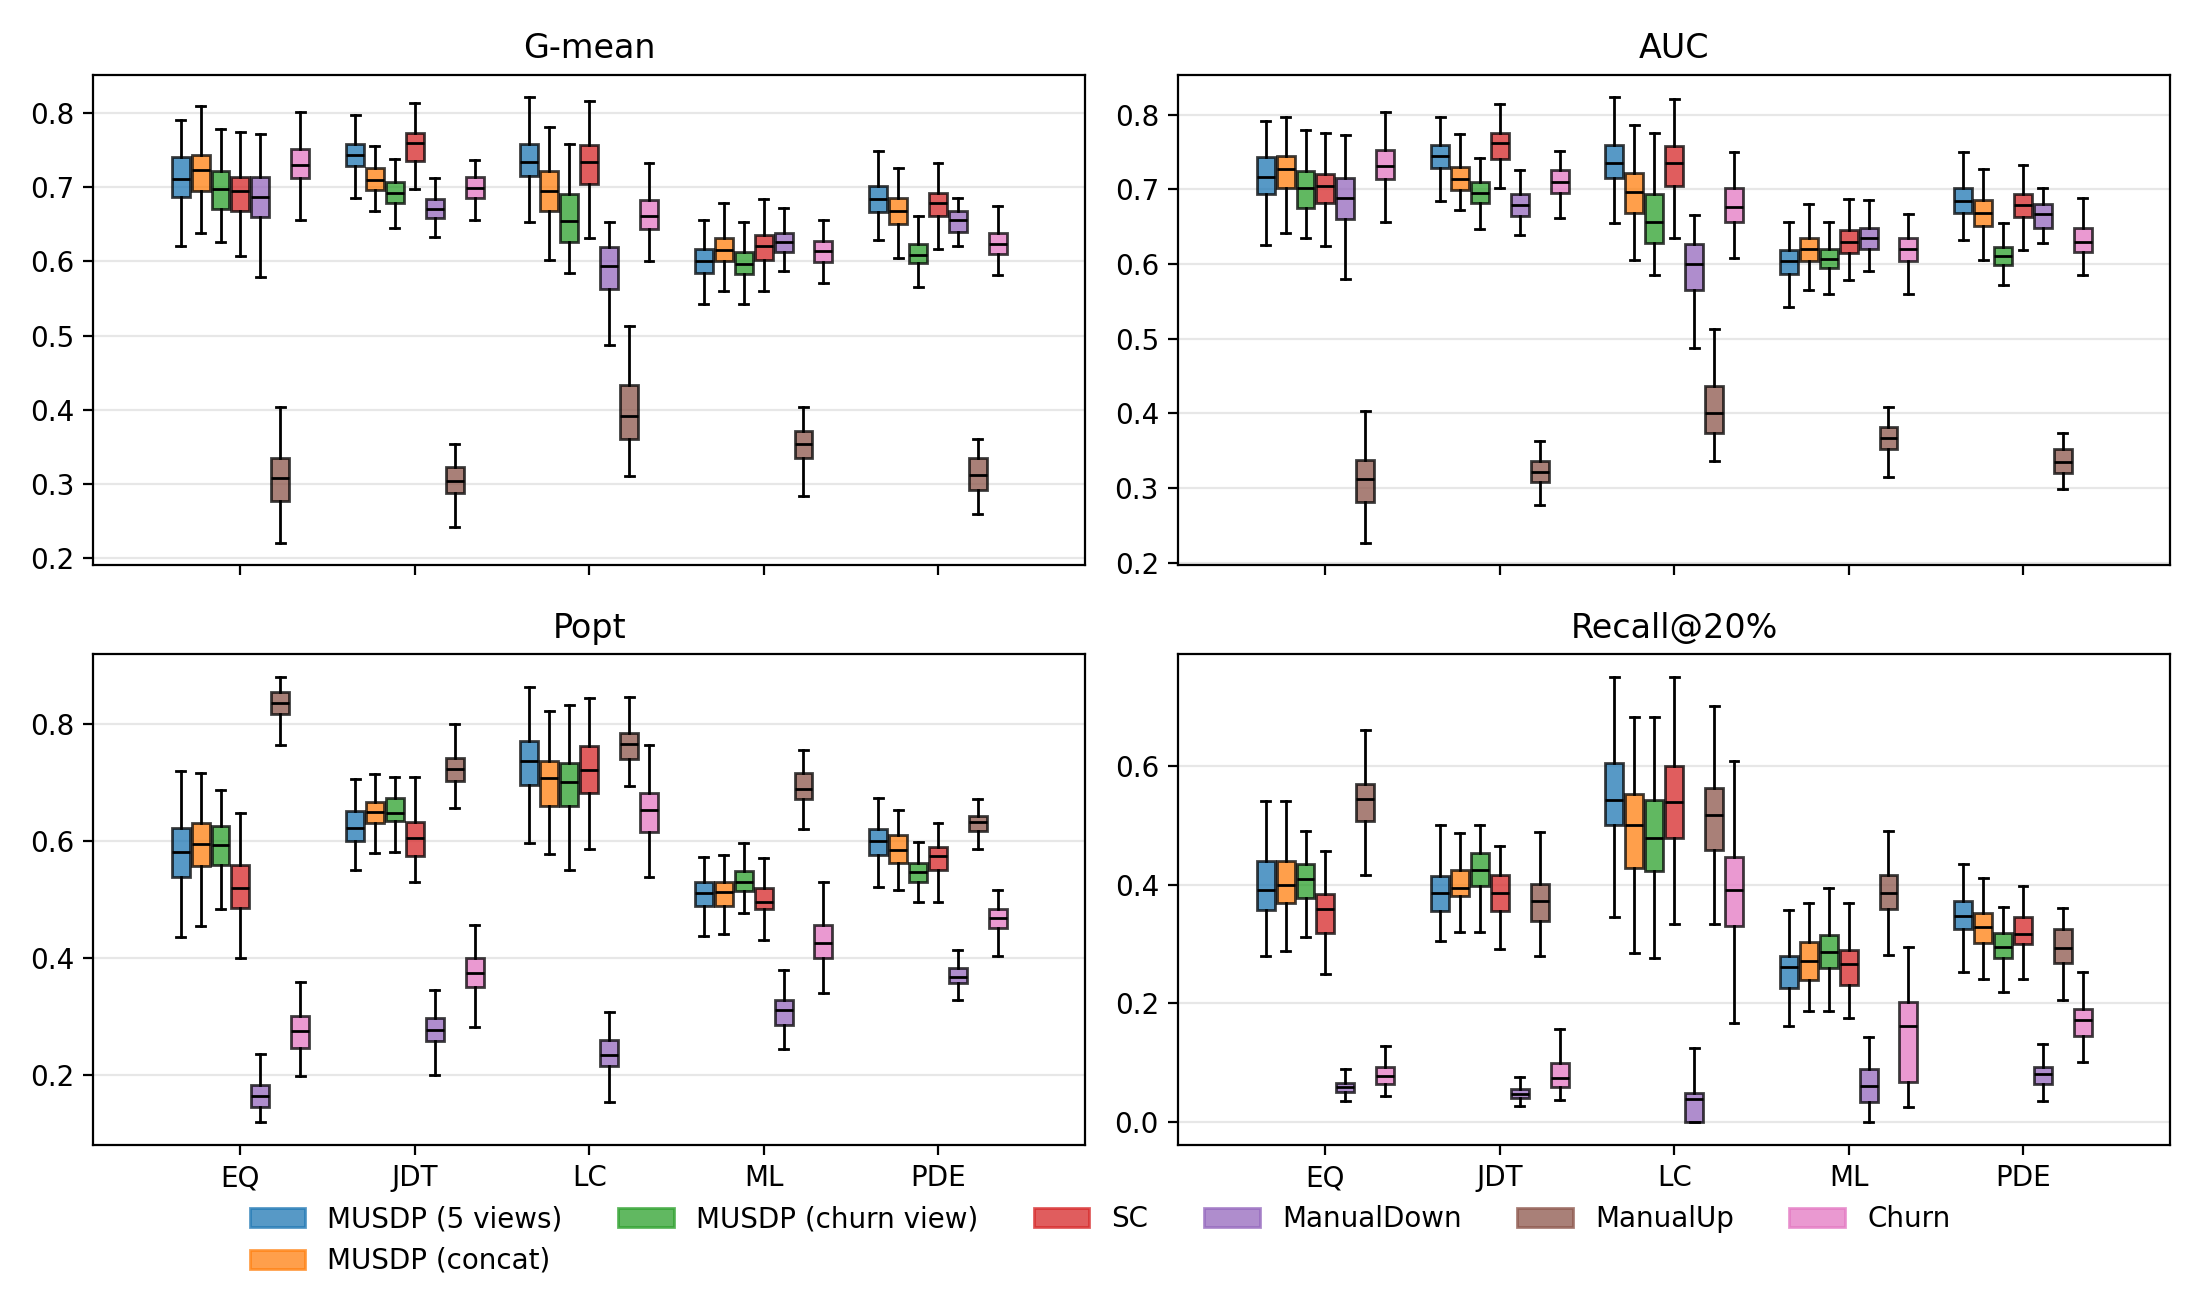
\includegraphics[width=\textwidth]{fig_aeeem_comparison.png}
\caption{Distribution over 100 bootstrap rounds for each AEEEM system.}
\label{fig:aeeem}
\end{figure*}

Tables~\ref{tab:aeeem-overall} and~\ref{tab:aeeem-systems} and
Fig.~\ref{fig:aeeem} give the results. MUSDP-5V has the best overall mean rank
and the highest median G-mean (0.711) and AUC (0.716), but the lead is small
and not uniform: SC is 0.016 G-mean behind overall, beats MUSDP-5V on JDT and
ML ($\delta=0.28$ and $0.42$, $p<0.05$) and does not differ on LC.

\emph{Multiview structure.} MUSDP-concat, which keeps the same metrics in one
view, loses to MUSDP-5V on JDT, LC and PDE (G-mean 0.018 to 0.037 lower,
$\delta=-0.37$ to $-0.69$), is level on EQ (negligible $\delta$) and is better
on ML. The five-view structure helps on three of the five systems.

\emph{Churn signal.} A single churn metric reaches a median G-mean of 0.662,
93\% of MUSDP-5V. It beats ManualDown on EQ, JDT and LC ($\delta=0.67$ to
$0.90$) and MUSDP-5V on EQ (0.731 vs 0.711) and ML (0.614 vs 0.600); its rank
AUC is 0.68 to 0.81. Summing all 17 churn metrics does not improve on it.

\emph{Measures disagree.} ManualUp has the best Popt on every system (median
0.722) and the worst G-mean (0.312). Churn and ManualDown inspect large classes
first and score low on Recall@20\% (0.162 and 0.059), while the same churn
metrics clustered by MUSDP reach Popt 0.593. ML has the lowest best G-mean
(0.626, by ManualDown), and no method leads on all five systems. MUSDP's two
labelling strategies produced identical labels in all 1500 rounds: majority
voting always chose the smaller cluster.

\subsection{Interpretation and validity}

On AEEEM the evidence supports a weaker version of the paper's claim: MUSDP
has the best median classification scores, but its overall margin is 0.016
G-mean over SC and 0.049 over a one-metric churn ranking, and both baselines
beat it on some systems. The strongest threat is class size. LOC is the effort
in Popt and Recall@20\%, and churn and most metrics grow with size.
Effort-aware scores mostly reward inspecting small classes first: ManualUp
wins Popt by doing only that, and binary methods get part of the same benefit
from the density ordering. Effort-aware differences may therefore come from
size ordering rather than from the clustering. Other threats: the fixed 50\%
cut-off sets the G-mean and AUC of the ranking methods; held-out samples
overlap between rounds, so Wilcoxon $p$-values are optimistic and effect sizes
are the more reliable figure; MUSDP results are preliminary runs of Member 2's
code.

\subsection{Remaining work: Comparison Part}

Merge Member 2's final MUSDP configurations (every single view and drop-one
views); rank methods with NPSKESD, the paper's test; and control for size with
a churn-density baseline, results by size stratum, and a sensitivity check of
the 50\% cut-off.

\textbf{Contributions (Emmanuel Omole).} AEEEM loader and view check; SC,
ManualDown, ManualUp, Churn and ChurnSet on AEEEM; one evaluation for all
methods; runner, summary tables, paired tests and figure; 212 validation tests
and the end-to-end check against the paper (168 of 168 values reproduced); the 100-round runs; the
\texttt{rank\_measure} issue; \texttt{test/run\_aeeem.py} made to read the
ARFF files and run on macOS, with identical results.
